\section{Results and Analysis} \label{sec:results}
% 1. Accuracy (F1 + MCC) auf SICK und eSNLI einzeln nach Kategorien
% 2. Auf Bias überprüfen: Vergleich vom Modell für wichtig erachtete Token mit von Menschen als wichitg erachtete Tokens
% Visualisierungen:
% - Confusion Matrix (Gentrennt nach Phänomenen)
% - Tabellen Interpretability Metriken (siehe ferret)
In this section the results of our experiments are described and thoroughly analyzed. The results are grouped according to the hypotheses they support.

\subsection{Testing H1}

\begin{table}[ht!]
    \centering
    \caption{Prediction performance when using prompting with different word groups on the \acs{SICK} dataset. The best result is shown in \textbf{bold} and the second-best is \underline{underlined}.}
    \begin{tabular}{l c c}
        \toprule
        \multicolumn{1}{c}{Word Group} & \acs{MCC} & $\text{F}_1$ \\
        \midrule
        A Priori & $\underline{25.51}\%$ & $\mathbf{54.31\%}$ \\
        Simple & $20.56\%$ & $\underline{34.40\%}$ \\
        Tuned & $\mathbf{29.11\%}$ & $34.08\%$ \\
        \bottomrule
    \end{tabular}
\end{table}

\subsection{Testing H2}
Figure~\ref{fig:metric-heatmap-phenomena-mcc} depicts the \acs{MCC} scores for our Base model separated by linguistic phenomena. As can be seen in the figure, there are disparities between different phenomena. Antonyms and numerals have the largest disparity of $\geq 0.1$. The Base model detects the phenomena antonyms, co-hyponyms and quantifiers best, while it detects numerals, hypernyms and hyponyms worst. The smallest difference between phenomena is between hypernyms and hyponyms, with a difference of $0.0077$.

Disparities between phenomena indicate a bias of the model towards certain phenomena. As can be clearly seen in figure~\ref{fig:metric-heatmap-phenomena-mcc}, the Base model is biased towards antonyms, co-hyponyms and quantifiers.

Figure~\ref{fig:ferret-sample} shows the explanations for the fine-tuned model's classification of a sample from the validation split of the \ac{e-SNLI} dataset obtained using ferret \cite{ferret}. It can be seen that the meaning of the quantifiers in this sample is not considered by the model: The usage of quantifiers in this sample makes it a contradiction but the model attaches high importance only to the quantifier \enquote{all} whereas \enquote{several} has very low importance to the model. The existence of such samples where the model only poorly captures the importance of quantifiers shows that the model is biased after fine-tuning on \ac{MultiNLI}.

\begin{figure*}[h!]
    \centering
    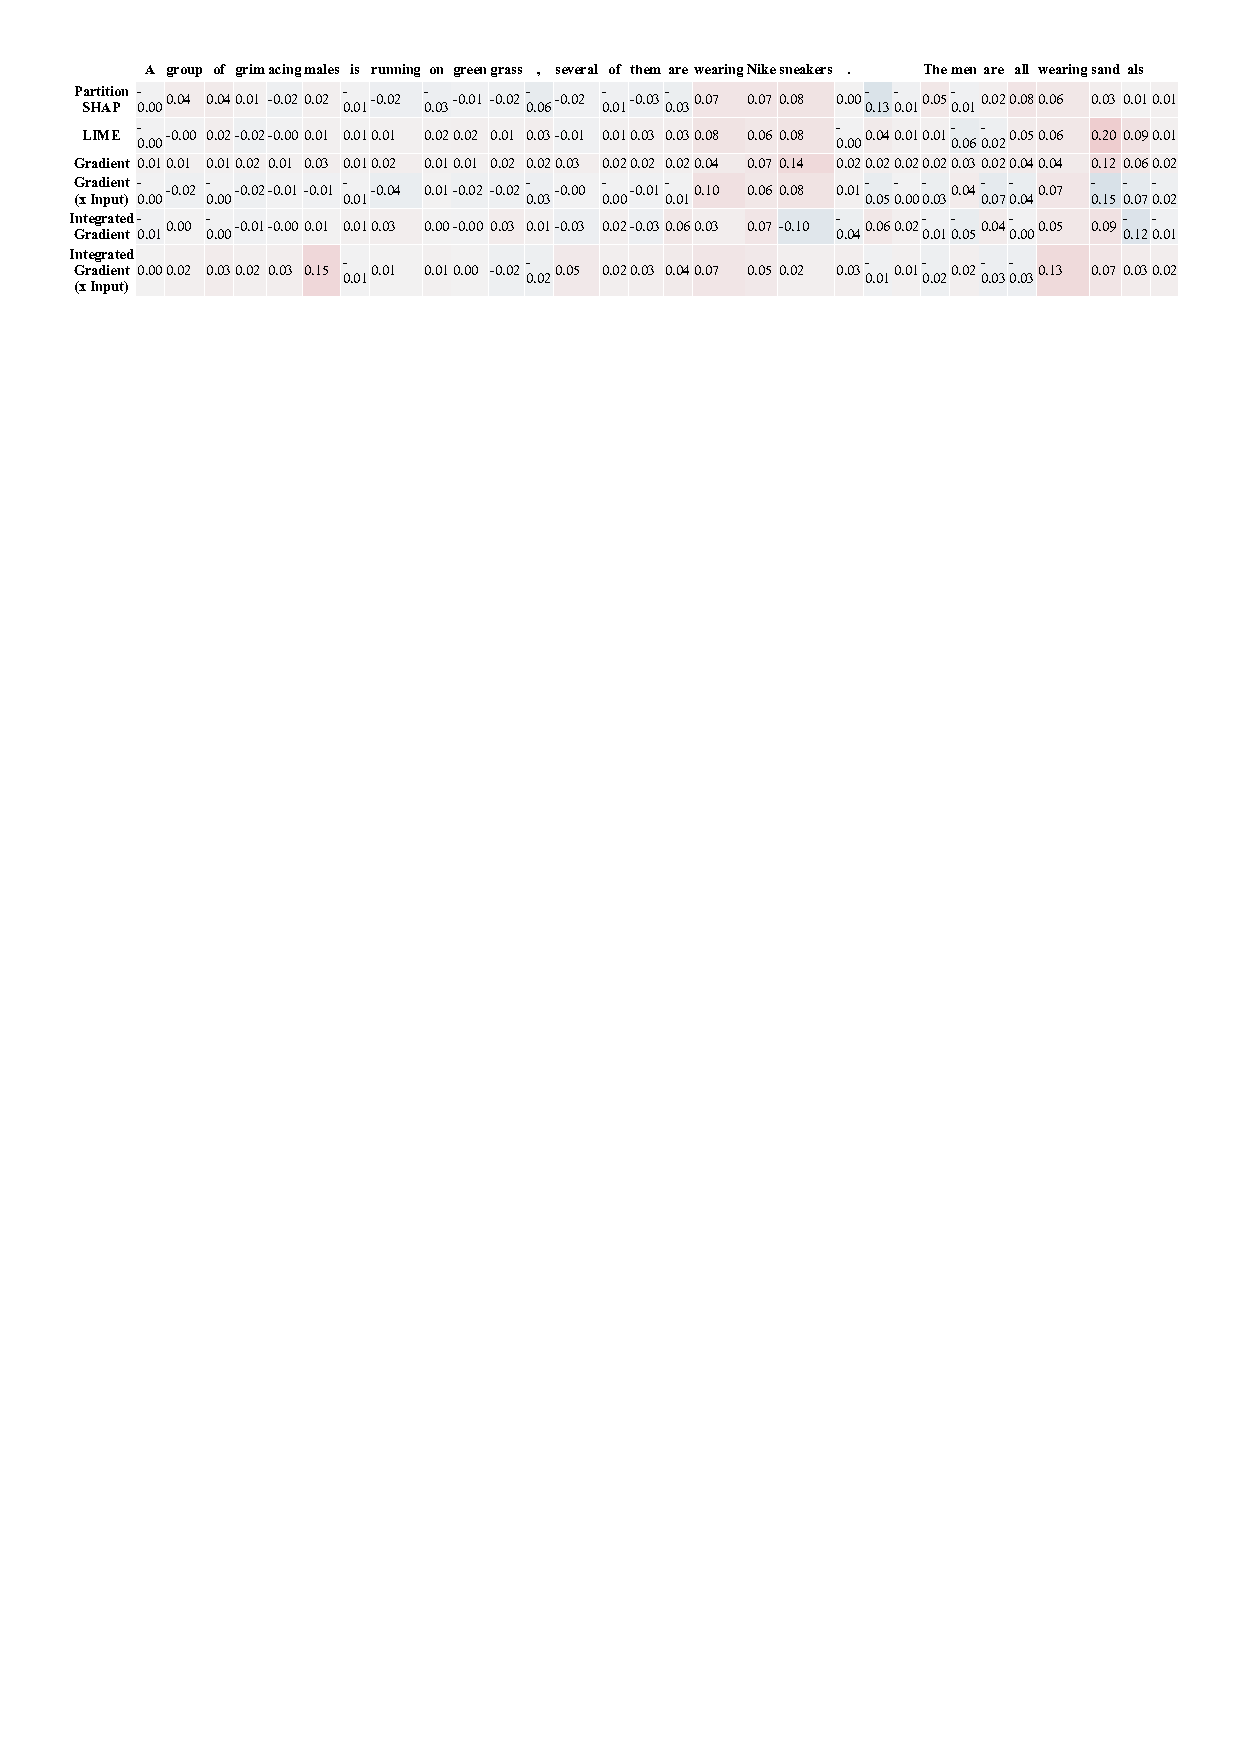
\includegraphics[width=\textwidth]{./images/ferret_sample.pdf}
    \caption{Example of a bad explanation}
    \label{fig:ferret-sample}
\end{figure*}

\subsection{Testing H3}

\begin{table}[ht!]
    \centering
    \caption{Prediction performance of our fine-tuned models on the \acs{SICK} dataset. The best result is shown in \textbf{bold} and the second-best is \underline{underlined}.}
    \begin{tabular}{l c c}
        \toprule
        \multicolumn{1}{c}{Model} & \acs{MCC} & $\text{F}_1$ \\
        \midrule
        Base & $49.49\%$ & $56.60\%$ \\
        Hypothesis-Only\tablefootnote{Average of three runs with different seeds} & $14.13\%$ & $40.02\%$ \\
        Filtered $2/3$ & $46.21\%$ & $54.12\%$ \\
        Filtered $2/3$ longer & $36.17\%$ & $52.85\%$ \\
        Filtered $3/3$ & $48.73\%$ & $56.94\%$ \\
        Filtered $3/3$ longer & $\mathbf{52.31\%}$ & $\mathbf{62.04\%}$ \\
        Ensembled & $\underline{51.65\%}$ & $\underline{59.88\%}$ \\
        Recast & n/a & n/a \\
        \bottomrule
    \end{tabular}
\end{table}

\subsection{Testing H4}
Figure~\ref{fig:metric-heatmap-phenomena-mcc} depicts the \ac{MCC} scores separated by linguistic phenomena for our model trained on different datasets as described in \autoref{sub:experiments-h4} to show the different predictive performance of the models.

\begin{figure}[ht]
    \centering
    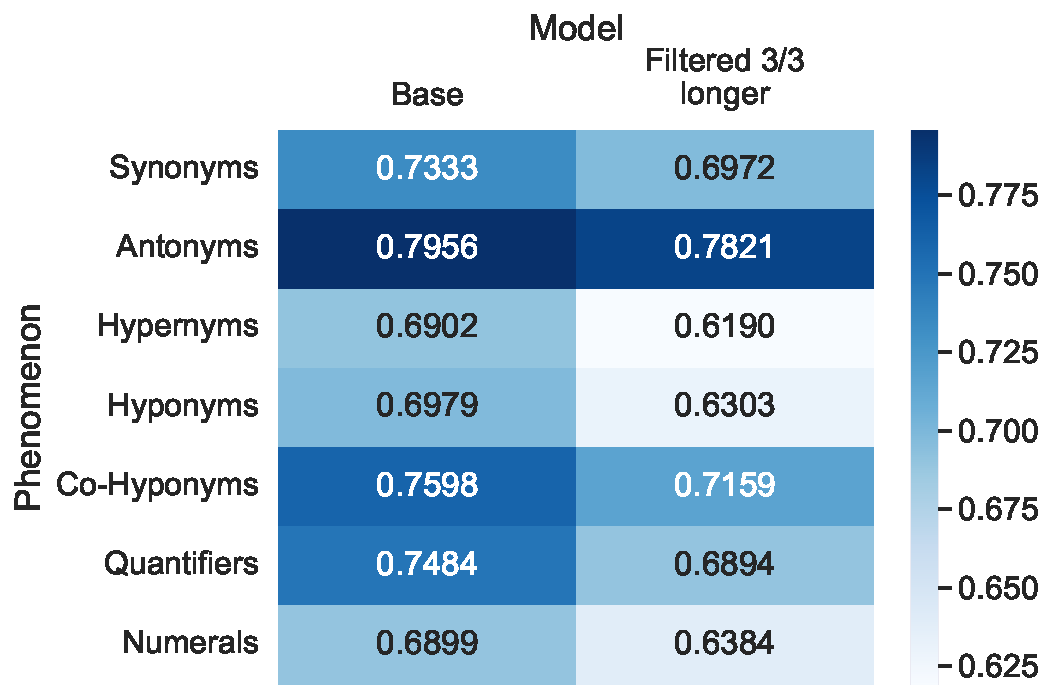
\includegraphics[width=0.9\columnwidth]{./images/metric_heatmaps_phenomena/important_words/matthews_correlation.pdf}
    \caption{Matthews Correlation Coefficients for the model trained on different datasets separated by linguistic phenomena}
    \label{fig:metric-heatmap-phenomena-mcc}
\end{figure}

The Hypothesis-Only model shows the expected poor performance but performs comparably well on samples that contain antonyms which indicates a bias in these samples as the model cannot detetct the presence of an antoymn for the right reasons without knowing the premise. The improved performance of the Filtered 3/3 longer model shows that this bias can be mitigated by the naive approach of removing the biased samples.

The Hypothesis-Only model also performs better on samples that contain quantifiers which indicates a bias also in these samples. As opposed to antonyms, the Filtered 3/3 longer model performs slightly worse on quantifiers than the Base model. Thus, it is not sufficient to remove the biased samples to increase performance on quantifiers. A reason for this behavior might be the greater complexity of quantifiers compared to antonyms. To increase the model's performance on quantifiers nevertheless, we collect additional training samples containing quantifiers.

\subsection{Testing H5}
